\documentclass{article}

\usepackage[T1]{fontenc}
\usepackage[polish]{babel}
\usepackage[utf8]{inputenc}
\usepackage{graphicx}
\usepackage{subcaption}

\title{%
\big Rozwiązywanie równania \\ macierzowego $AX=B$ \\
\large\\ za pomocą rozkładu Cholesky'ego-Banachiewicza}
\author{Tymoteusz Kwieciński}
\date{Grudzień 2022}

\begin{document}

\maketitle

\tableofcontents
\newpage

\section{Opis zadania}

Moim zadaniem było rozwiązywanie równania macierzowego $AX = B$, gdzie $A \in \mathbf{R}^{n \times n}$ jest macierzą symetryczną oraz dodatnio określoną, zaś macierz $B \in \mathbf{R}^{n \times m}, \quad m \geq 1$, przy pomocy metody Cholesky'ego-Banachiewicza. 


\section{Opis używanej metody}

% tutaj jeszcze może jakies matematyczne uzasadnienie - ale dowolnie

Metoda Cholesky'ego-Banachiewicza rozwiązywania równania macierzowego $AX = B$, polega na rozkładzie macierzy symetrycznej, dodatnio określonej $A$ na iloczyn macierzy $L \cdot L^T$, gdzie macierz $L$ jest macierzą dolnotrójkątną.

Po rozłożeniu macierzy $A$ na iloczyn macierzy $L \cdot L^T$ należy rozwiązać dwa proste równania macierzowe:

\begin{enumerate}
    \item $LY = B$, $L$ jest macierzą dolnotrójkątną.
    \item $L^TX = B$, $L^T$ jest macierzą górnotrójkątną.
\end{enumerate}

Wówczas macierz $X$ jest szukanym rozwiązaniem równania, gdyż spełnia ona równanie:
$$ AX = L (L^T X) = L Y = B$$



\section{Sposób implementacji}

Zadanie zostało zaimplementowane w programie MATlab. 
Program składa się z kilku funkcji, które wzajemnie składają się na rozwiązanie zadania.


\section{Sposób pomiaru błędu}
Aby zweryfikować poprawność stosowanego przeze mnie algorytmu ustaliłem prosty sposób weryfikacji błędu otrzymywanej macierzy $X$. 

Miarą błędu było odchylenie przeciętne wartości macierzy $AX$ oraz macierzy $B$, gdzie macierz $X$ jest znalezionym rozwiązaniem równania $AX=B$.

\newpage
\section{Przykłady}
Aby sprawdzić zachowanie, poprawność i wydajność napisanej przeze mnie funkcji rozwiązującej równanie macierzowe $AX=B$ przy użyciu metody Cholesky'ego- Banachiewicza, przetestowałem ją na kilku przykładowych macierzach.

Dodatkowo wyniki były porównywane z wynikami funkcji rozwiązującej równanie $AX=B$ przy użyciu wbudowanej funkcji programu $MATlab$ odwracającej macierz - $inv()$. Funkcja rozwiązywała układ równań szukając wpierw macierzy $A^{-1}$ - odwrotnej do $A$, a następnie mnożąc ją lewostronnie z macierzą $B$.

\subsection*{Przykład 1.}
Macierz $A$ jest jednostkowa o wymiarach $3 \times 3$, zaś $B$ macierzą o wymiarach $3 \times 4$ o wartościach losowych.

$$ A =\pmatrix{
    1 & 0 & 0 \cr
    0 & 1 & 0 \cr
    0 & 0 & 1 
} $$
$$B = \pmatrix{
0.5377  &  0.8622  & -0.4336  &  2.7694 \cr
    1.8339 &   0.3188  &  0.3426   &-1.3499 \cr
   -2.2588  & -1.3077 &   3.5784    &3.0349
}$$

W tym przypadku, algorytm sprawdził się bardzo dobrze. Rozłożył macierz $A$ dokładnie na iloczyn dwóch macierzy jednostkowych, a także ustalił precyzyjnie $X = B$.
\\
Podobnie dobrze sprawdziła się również funkcja używająca wbudowaną funkcję programu MATlab \textit{inv}.

\newpage
\subsection*{Przykład 2.}

Macierz $A$ jest macierzą symetryczną, dodatnio określoną o wymiarach $3 \times 3$, gdzie na miejscu $(i,j)$ macierzy $A$ stoi największy wspólny dzielnik $i$ oraz $j$. $B$ jest macierzą jednostkową o wymiarach $3 \times 3$.


$$
A = \pmatrix{
     1  &   1  &   1 \cr
     1  &   2  &   1 \cr
     1  &   1  &   3
}
$$
$$ B =\pmatrix{
    1 & 0 & 0 \cr
    0 & 1 & 0 \cr
    0 & 0 & 1 
} $$

W tym przypadku napisana przeze mnie metoda zwróciła macierz $X$ będącą bardzo blisko poprawnego wyniku. Odchylenie przeciętne odpowiadających współczynników wynosiło 

\begin{center}
\begin{tabular}{ |c||c|c| }
 \hline
 Badana metoda & Cholesky-Banachiewicz & wbudowana funkcja \textit{inv}   \\
  \hline
    Przybliżony błąd & $10^{-16}$ & 0 \\
 \hline
\end{tabular}
\end{center}

\subsection*{Przykład 3.}
Przykład numer 3 ma na celu sprawdzenie jak zaimplementowane funkcje radzą sobie z napotkanymi błędami. W tym przypadku podana macierz $A$ nie jest dodatnio określona.



$$
A = \pmatrix{
     1  &   1  &   1 \cr
     1  &   1  &   1 \cr
     1  &   1  &   1
}
$$
$$ B =\pmatrix{
    1 & 0 & 0 \cr
    0 & 1 & 0 \cr
    0 & 0 & 1 
} $$

Zgodnie z przewidywaniami, algorytm nie poradził sobie z rozwiązaniem równania, gdyż rozwiązanie równania $AX = B$ z takimi danymi jak wyżej nie istnieje.

\newpage

\section{Dalsze przykłady}
W tym oraz następnych przykładach analizować będę wielokrotne przykłady - to znaczy przy pomocy funkcji $gallery$ programu MATlab generowałem coraz większe macierze $A$ o wymiarach $n \times n$ dla zwiększających się wartości $n$. W ten sposób można łatwo porównać dokładność metody wykorzystującej wbudowaną funkcję programu MATlab oraz tą napisaną przeze mnie.

Co więcej takie podejście pokazuje, że zaimplementowana przeze mnie funkcja rzeczywiście działa - na przykładach różnego typu i rozmiarów.

\subsection*{Przykład 4.}

Macierz $A$ o wymiarach $n \times n$ jest macierzą najmniejszej wspólnej wielokrotności - $A$ jest macierzą symetryczną, dodatnio określoną o wymiarach $3 \times 3$, gdzie na miejscu $(i,j)$ macierzy $A$ stoi największy wspólny dzielnik $i$ oraz $j$. Macierz $B$ jest macierzą o wymiarach $n \times 4$ o współczynnikach naturalnych nie większych niż 10, generowana losowo.


\begin{figure}[!ht]
\centering
  \centering
  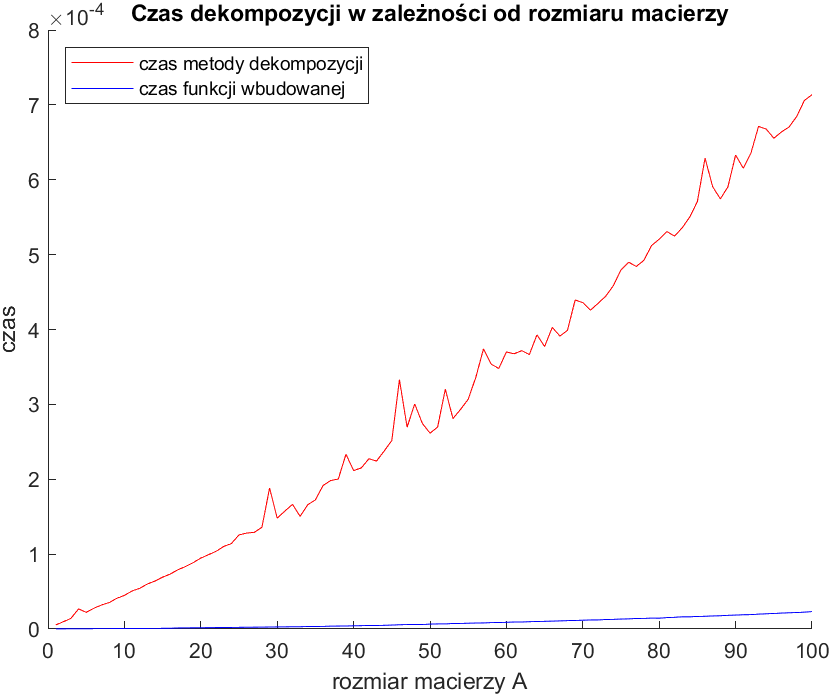
\includegraphics[width=9cm]{wykresy/przyklad4_1.png}
  \caption{Wykres czasu wykonywania dekompozycji różnymi metodami\\
  dla macierzy najmniejszej wspólnej wielokrotności }
  \label{fig:sub1}
\label{fig:test}
\end{figure}


\begin{figure}[!ht]
\centering
  \centering
  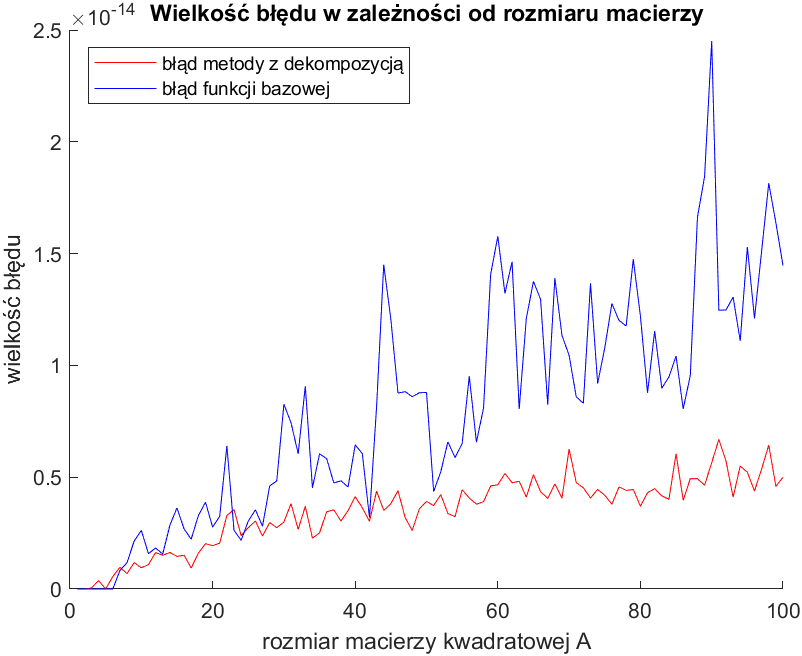
\includegraphics[width=9cm]{wykresy/przyklad4.png}
  \caption{Wykres odchylenia przeciętnego iloczynu znalezionego rozwiązania \\
  dla macierzy najmniejszej wspólnej wielokrotności i losowej macierzy B o 4 kolumnach}
  \label{fig:sub1}
\label{fig:test}
\end{figure}

Jak widać, zaimplementowana przez nas metoda wykorzystująca dekompozycje sprawuje się trochę lepiej dla macierzy większych wymiarów, niż wbudowana metoda. Jest jednak od niej znacząco wolniejsza i mniej stabilna czasowo.


\subsection*{Przykład 5.}
Podobnie jak w poprzednim przykładzie macierz $A$ jest macierzą najmniejszej wspólnej wielokrotności i losowej macierzy $B$ o wartościach naturalnych nie większych od 100, tym razem macierz $B$ ma 100 kolumn


\begin{figure}[!ht]
\centering
  \centering
  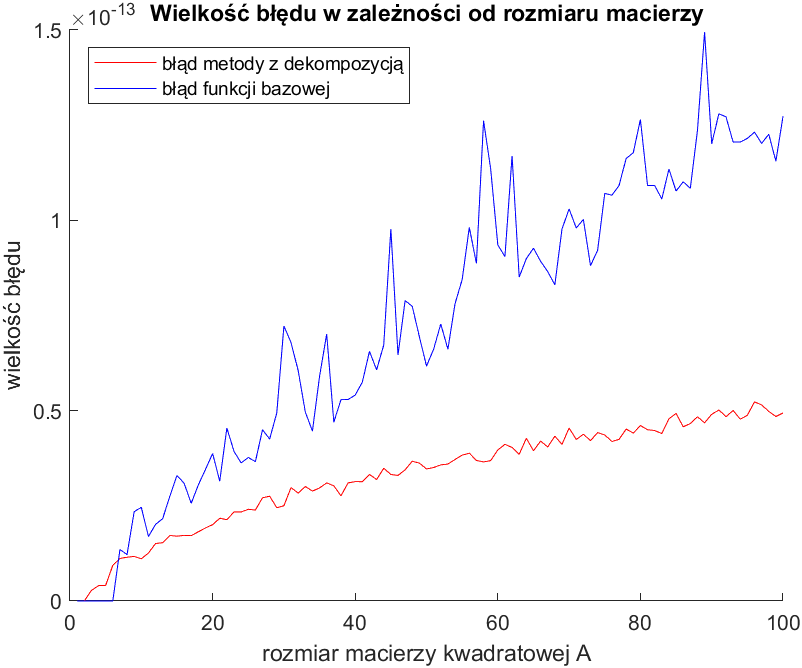
\includegraphics[width=9cm]{wykresy/przyklad5.png}
  \caption{Wykres odchylenia przeciętnego iloczynu znalezionego rozwiązania \\
  dla macierzy najmniejszej wspólnej wielokrotności i losowej macierzy B o 100 kolumnach}
  \label{fig:sub1}
\label{fig:test}
\end{figure}

Podobnie jak w poprzednim przykładzie wartość błędu jest mniejsza w przypadku metody używającej dekompozycję, ale jej czas działania jest dłuższy.

\newpage

\subsection*{Przykład 6.}

Macierz $A$ o wymiarach $n \times n$ jest dodatnio określoną, symetryczną macierzą Lehmera. Macierz $B$ jest macierzą o wymiarach $n \times 100$ o współczynnikach losowych z rozkładu normalnego.



\begin{figure}[htp]
\centering
  \centering
  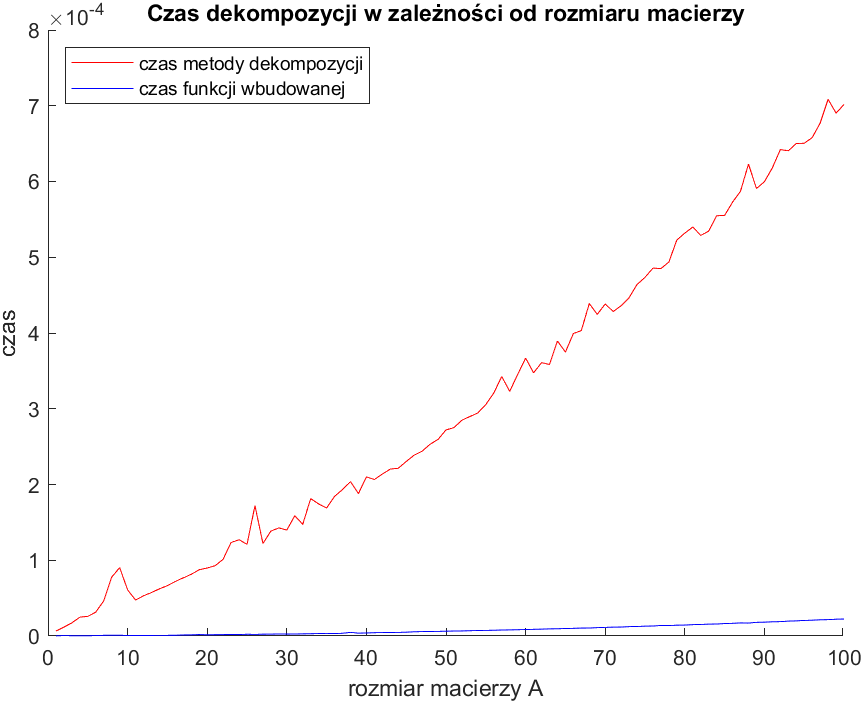
\includegraphics[width=9cm]{wykresy/przyklad6_1.png}
  \caption{Wykres czasu wykonywania dekompozycji różnymi metodami dla macierzy Lehmera}
  \label{fig:sub1}
\label{fig:test}
\end{figure}

\begin{figure}[htp]
\centering
  \centering
  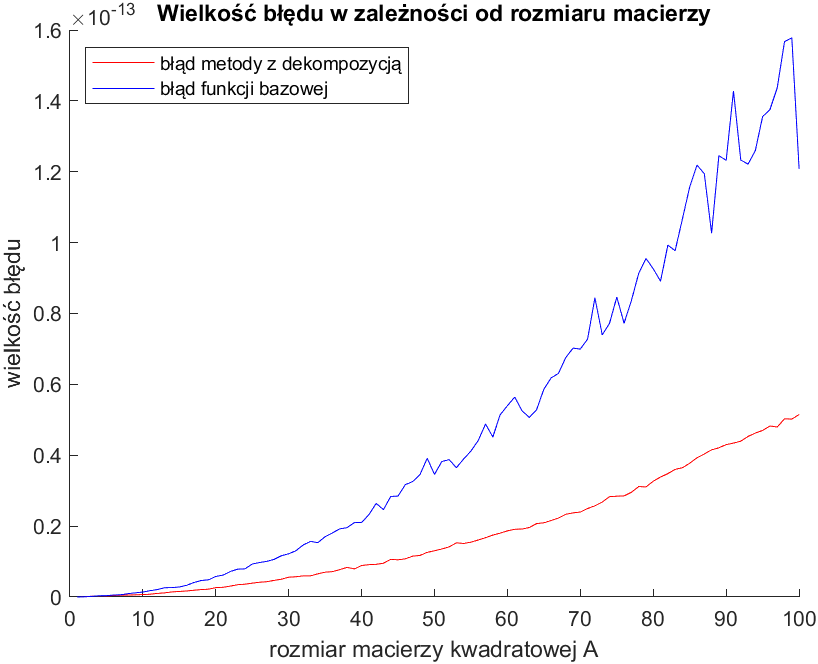
\includegraphics[width=9cm]{wykresy/przyklad6.png}
  \caption{Wykres odchylenia przeciętnego iloczynu znalezionego rozwiązania \\
  dla macierzy Lehmera i losowej macierzy B o 100 kolumnach}
  \label{fig:sub1}
\label{fig:test}
\end{figure}

Ponownie, zaimplementowana przeze mnie metoda daje bardziej dokładne rezultaty, ale sprawowała się znacznie wolniej.
\newpage
\subsection*{Przykład 7}
W tym przypadku macierz $A$ jest macierzą rzadką o współczynnikach tylko na trzech diagonalach o wymiarach $n \times n$ gdzie $n$ jest nie większe niż 500, zaś macierz $B$ jest macierzą o wymiarach $n \times 200$ o współczynnikach losowych z rozkładu normalnego.




\begin{figure}[htp]
\centering
  \centering
  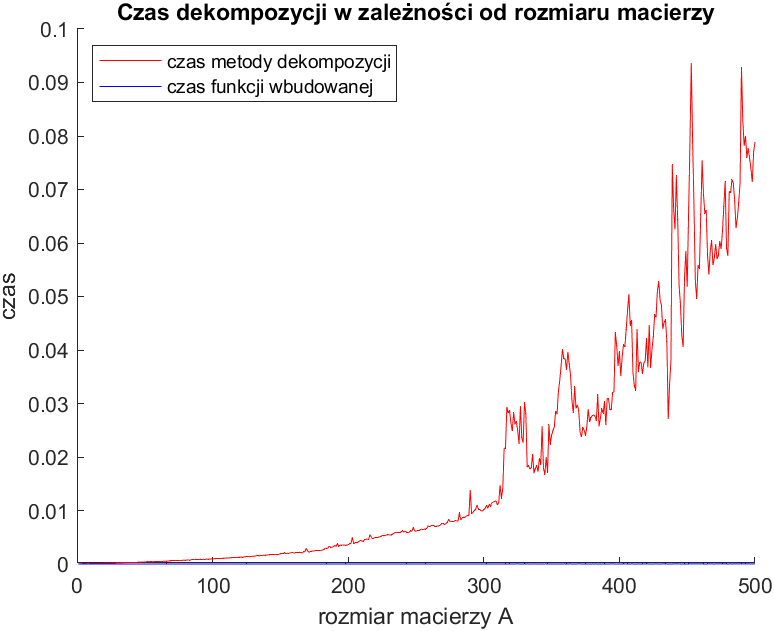
\includegraphics[width=9cm]{wykresy/przyklad7_1.png}
  \caption{Wykres czasu wykonywania dekompozycji różnymi metodami dla rzadkiej macierzy}
  \label{fig:sub1}
\label{fig:test}
\end{figure}


\begin{figure}[htp]
\centering
  \centering
  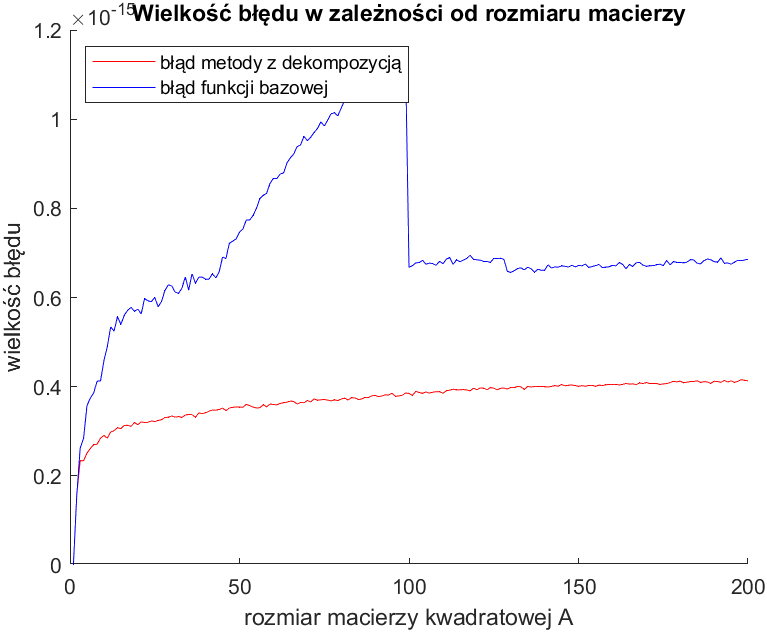
\includegraphics[width=9cm]{wykresy/przyklad7.png}
  \caption{Wykres odchylenia przeciętnego iloczynu znalezionego rozwiązania \\
  dla macierzy rzadkiej i losowej macierzy B o 200 kolumnach}
  \label{fig:sub1}
\label{fig:test}
\end{figure}

Ponownie, zaimplementowana funkcja zwróciła dokładniejsze wyniki. Również w tym przypadku jej czas działania był znacznie dłuższy

\newpage
\section{Jeszcze więcej przykładów}

Aby sprawdzić wydajność zaimplementowanej funkcji wykorzystującej dekompozycję, zmierzyłem i porównałem czasy wykonywania poszczególnych wywołań obliczania równania $AX = B$ za pomocą napisanej przeze mnie funkcji oraz funkcji wykorzystującej odwracanie macierzy.


\subsection*{Przykład 8}
Macierz $A$ jest macierzą symetryczną, dodatnio określoną o wymiarach $3 \times 3$, gdzie na miejscu $(i,j)$ macierzy $A$ stoi największy wspólny dzielnik $i$ oraz $j$. $B$ jest macierzą jednostkową o wymiarach $3 \times 3$.


$$
A = \pmatrix{
     1  &   1  &   1 \cr
     1  &   2  &   1 \cr
     1  &   1  &   3
}
$$
$$ B =\pmatrix{
    1 & 0 & 0 \cr
    0 & 1 & 0 \cr
    0 & 0 & 1 
} $$

W tym przypadku napisana przeze mnie metoda zwróciła macierz $X$ będącą bardzo blisko poprawnego wyniku. Czas działania poszczególnych funkcji wynosił

\begin{center}
\begin{tabular}{ |c||c|c| }
 \hline
 Badana metoda & Cholesky-Banachiewicz & wbudowana funkcja \textit{inv}   \\
  \hline
    przybliżony czas działania & $10^{-5}$ & $10^{-6}$ \\
 \hline
\end{tabular}
\end{center}
Jak się okazuje funkcja wykorzystująca dekompozycję macierzy metodą Cholesky'ego-Banachiewicza jest odrobinę wolniejsza.
\subsection*{Przykład 9}
W tym przypadku macierz $A$ jest macierzą Lehmera  $100 \times 100$ zaś macierz $B$ jest macierzą o wymiarach $100 \times m$, gdzie $m$ jest nie większe niż 100, o współczynnikach losowych z rozkładu normalnego.

\begin{figure}[htp]
\centering
  \centering
  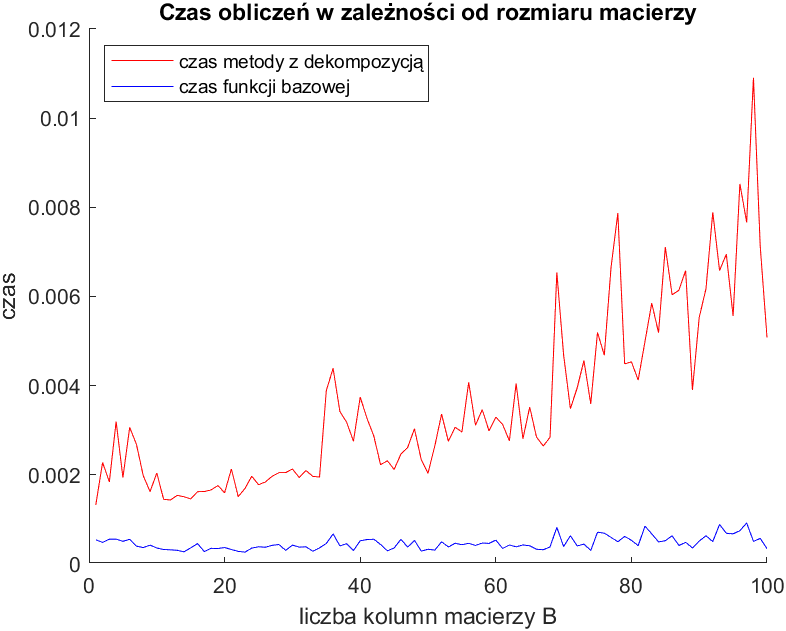
\includegraphics[width=9cm]{wykresy/przyklad9.png}
  \caption{Wykres odchylenia przeciętnego iloczynu znalezionego rozwiązania \\
  dla macierzy rzadkiej i losowej macierzy B o 200 kolumnach}
  \label{fig:sub1}
\label{fig:test}
\end{figure}


W tym przypadku funkcja wykorzystująca macierz odwrotną poradziła sobie lepiej niż zaimplementowana funkcja wykorzystująca dekompozycje Cholesky'ego-Banachiewicza, mimo że ta różnica była niewielka. 

\newpage

\subsection*{Przykład 10}
W tym przypadku macierz $A$ jest macierzą rzadką o współczynnikach tylko na trzech diagonalach o wymiarach $100 \times 100$, zaś macierz $B$ jest macierzą o wymiarach $100 \times m$,  gdzie $m$ jest nie większe niż 500 o współczynnikach losowych z rozkładu normalnego.

\begin{figure}[htp]
\centering
  \centering
  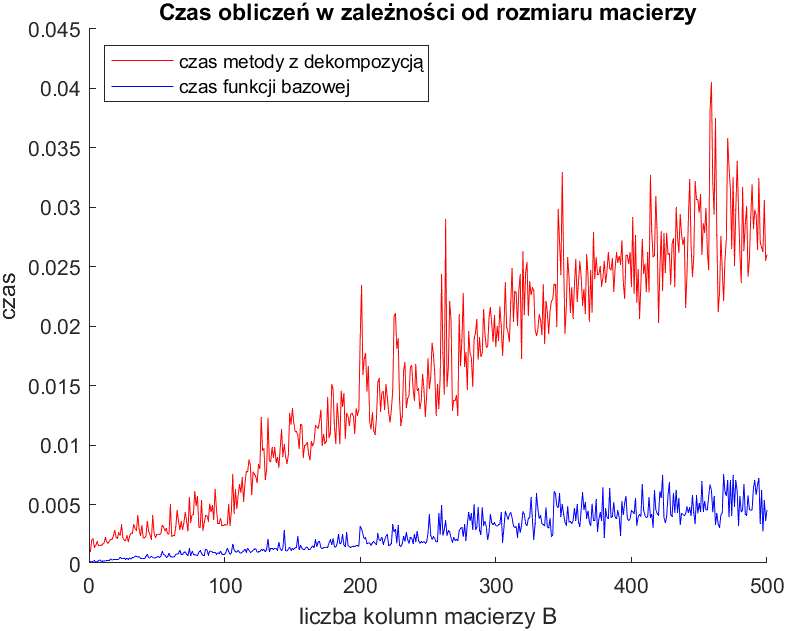
\includegraphics[width=9cm]{wykresy/przyklad10.png}
  \caption{Wykres czasu potrzebnego na rozwiązanie równania \\
  dla macierzy rzadkiej i losowej macierzy B}
  \label{fig:sub1}
\label{fig:test}
\end{figure}

W tym przypadku ponownie funkcja wykorzystująca macierz odwrotną poradziła sobie lepiej niż zaimplementowana funkcja wykorzystująca dekompozycje Cholesky'ego-Banachiewicza, mimo że ta różnica była niewielka. 

\newpage
\section{Podsumowanie}
Okazuje się, że zaimplementowana przeze mnie metoda, zarówno w przypadku dekompozycji jak i rozwiązywaniu równań macierzowych, mimo wektoryzacji, sprawuje się trochę wolniej niż funkcja wykorzystująca macierz odwrotną i wbudowaną funkcję programu MATlab.

Mimo to wydaje się bardzo dobrą funkcją do rozwiązywania równań zadanego typu, szczególnie, że zwracane wyniki są bardziej dokładne.

\section{Literatura}
\begin{itemize}
    \item Notatki z wykładu z przedmiotu Metody Numeryczne
    \item \textit{D. Kincaid, W. Cheney} - \textit{Analiza numeryczna} Warszawa 2005
\end{itemize}

\end{document}